\documentclass[12pt, letterpaper]{article}
\usepackage{graphicx}
\usepackage[a4paper, total={7in, 9in}]{geometry}
\usepackage{tikz}
\usepackage[utf8]{inputenc}
\usetikzlibrary{positioning}
\usepackage{fullpage, parskip, hyperref}

\title{Inteligencia Artificial - Problemas propuestos}
\author{Alumno: Marko Echevarria Narrea}
\date{}

\begin{document}

\tikzset{  a/.style={circle, draw, minimum size=1.5cm} }

\maketitle

\section{Ejercicio propuesto}

Considere una red neuronal Perceptrón Multicapa tal como la mostrada en la figura.

\begin{figure}[h!]
    \centering
    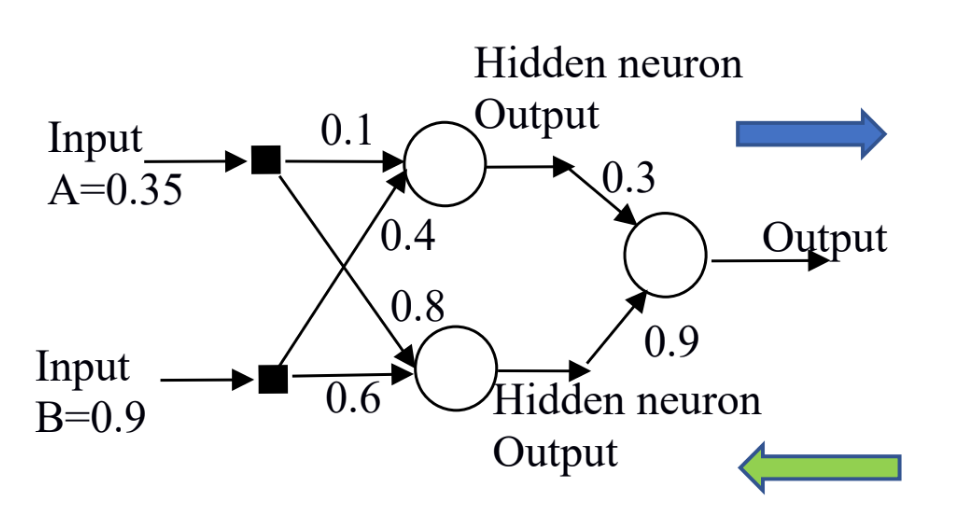
\includegraphics[width=0.8\linewidth]{image_problem.png}
    \label{fig:enter-label}
\end{figure}

Asuma que todas las neuronas de procesamiento usan como función de activación la logística sigmoide.

Responda:

\renewcommand{\theenumi}{\alph{enumi}}
\begin{enumerate}
    \item Realice la etapa forward (hacia adelante) de la red. El valor de salida deseado es 0.5.
    \item Realice la etapa backward (backpropagation o retropropagación del error) de la red. Considere una tasa de aprendizaje de 1 y, por razones de facilidad para la solución de este problema, no considere biases en la red.
    \item Realice una etapa forward (hacia adelante) más y comente el resultado que obtuvo respecto del anterior.
\end{enumerate}

Caso se requiera puede usar las siguientes expresiones matemáticas:

\[ \delta_k = ( t_k - y_k ) \times f'(u_k) \]
\[ \delta_j = ( \sum \delta_k - w_k ) \times f'(u_j) \]

Derivada de la funcion logistica sigmoide \( f'(u) = f(u) \cdot [ 1 - f(u) ] \)

\subsection*{Nota}

\renewcommand{\theenumi}{\arabic{enumi}}
    \begin{enumerate}
        \item No se han considerado biases en las neuronas ocultas ni en las de salida.
        \item En este problema los pesos de las conexiones entre las neuronas de entrada y las ocultas se simbolizan como wji, y los pesos de las conexiones entre estas neuronas y las neuronas de salida, se simbolizan como zkj.
    \end{enumerate}
\section{Resolucion}

\begin{center}
    \begin{tikzpicture}
        \node (input1) at (-3,0) {};
        \node (input2) at (-3,-4.5) {};
        \node[a] (a1)  {$i_1$}
            edge[<-] node[above, sloped, font=\small] {$x_1 = 0.35$} (input1);
        \node[a, below=30mm of a1] (a3)  {$i_2$}
            edge[<-] node[above, sloped, font=\small] {$x_2=0.9$} (input2);;
        \node[a, right=30mm of a1] (a2)  {$h_1$} 
            edge[<-] node[above, sloped, font=\small] {$w_{11} = 0.1$} (a1) 
            edge[<-] node[above, sloped, font=\small, pos=0.25] {$w_{12} = 0.4$} (a3);
        \node[a, below=30mm of a2] (a4)  {$h_2$} 
            edge[<-] node[above, sloped, font=\small,  pos=0.25] {$w_{21} = 0.8$} (a1) 
            edge[<-] node[below, sloped, font=\small] {$w_{22}$ = 0.6} (a3);
        \node[a, below right= 12mm and 30mm of a2] (a5)  {$y$} 
            edge[<-] node[below, sloped, font=\small] {$z_{11}$ = 0.6} (a2) 
            edge[<-] node[below, sloped, font=\small] {$z_{12}$ = 0.9} (a4);
    \end{tikzpicture}
\end{center}

\subsection*{Forward}

Suponemos que $x_i$ hace referencia a cada input de cada neurona de la capa de entrada 
\begin{center}
    $x_i=s_i$ entonces $x_1=s_1$ y $x_2=s_2$
\end{center}
\begin{center}
    $u_j$ : Entrada neta en la neurona 
\end{center}
\begin{center}
    $f(u_j)$: activación de la neurona
\end{center}
\begin{center}
    Primera neurona oculta: $u_1 = w_{11} \cdot x_1 + w_{12} \cdot x_2$ (regla de propagación)
\end{center}
\begin{center}
    Segunda neurona oculta: $u_2 = w_{21} \cdot x_1 + w_{22} \cdot x_2$ (regla de propagación)
\end{center}
\begin{center}
    Primera neurona oculta: $f(u_1)=\frac{1}{1+e^{u_1}}$ (regla de activación)
\end{center}
\begin{center}
    Segunda neurona oculta: $f(u_2)=\frac{1}{1+e^{u_2}}$ (regla de activación)
\end{center}
\begin{center}
    Entrada neta en primera neurona oculta: $(0.35 \cdot 0.1) + (0.9 \cdot 0.4) = 0.395$
\end{center}
\begin{center}
    Salida de la primera neurona oculta: 0.5975.
\end{center}
\begin{center}
    Entrada neta en segunda neurona oculta: $(0.9 \cdot 0.6) + (0.35 \cdot 0.8) = 0.82.$
\end{center}
\begin{center}
    Salida de la segunda neurona oculta: 0.6942.
\end{center}

\href{https://mattmazur.com/2015/03/17/a-step-by-step-backpropagation-example/}{Link de referencia}
\end{document}